\hsection{Installing PyCharm under Microsoft Windows}%
\label{sec:installingPyCharmWindows}%
%
\begin{figure}%
\centering%
%
\subfloat[][%
The download website \url{https://www.jetbrains.com/pycharm/download} for \pycharm.%
\label{fig:installingPyCharmWindows01download}%
]{\tightbox{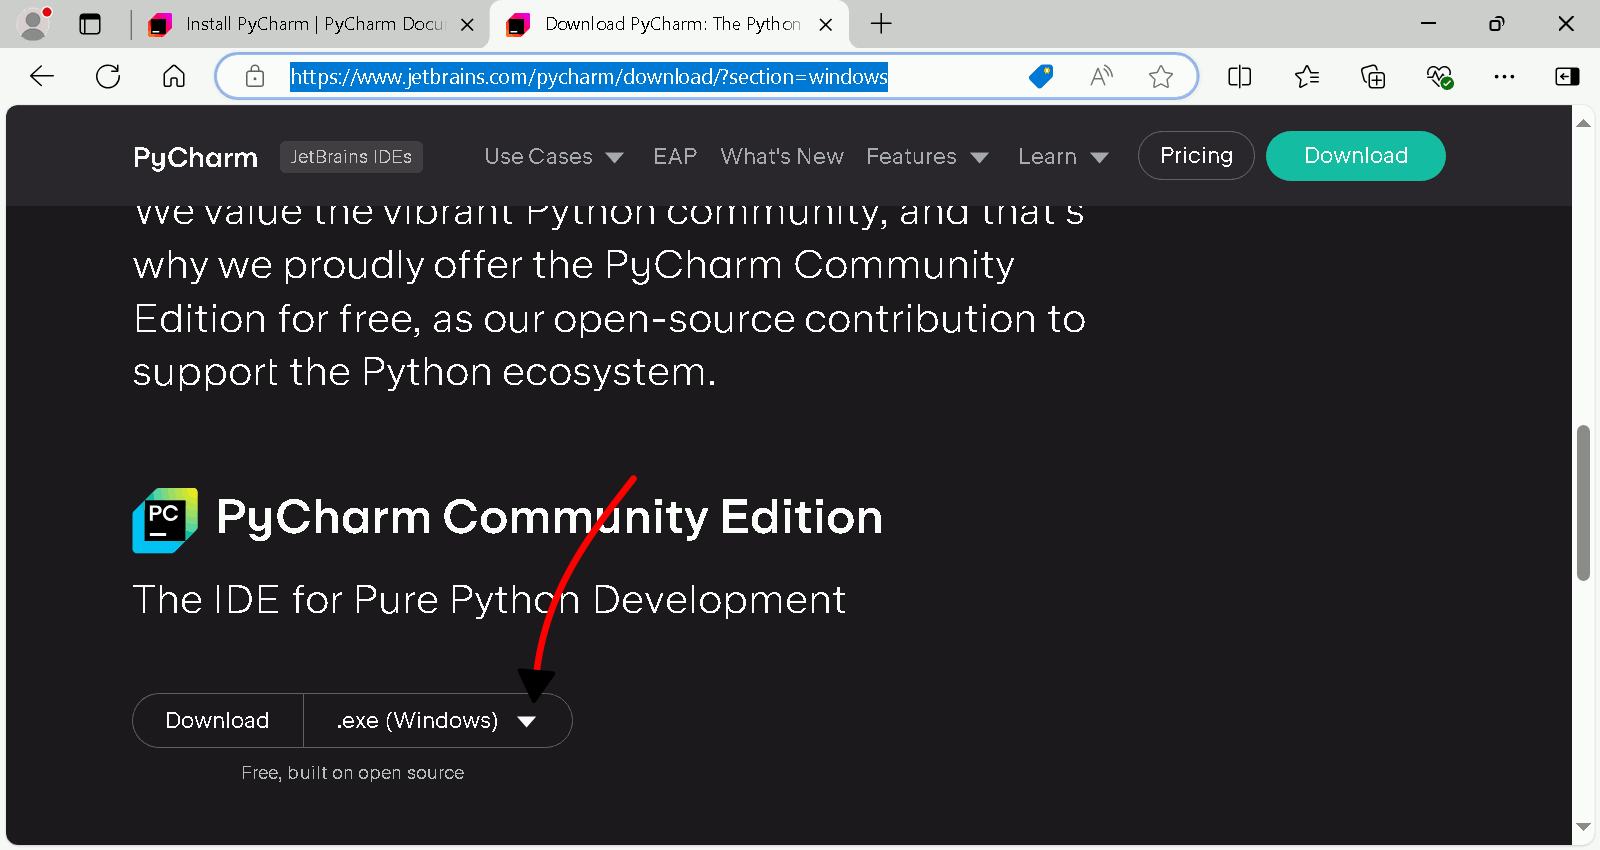
\includegraphics[width=0.47\linewidth]{\currentDir/installingPyCharmWindows01download}}}%
%
\hfill%
%
\subfloat[][%
Downloading the \pycharm\ Community Edition.%
\label{fig:installingPyCharmWindows02download}%
]{\tightbox{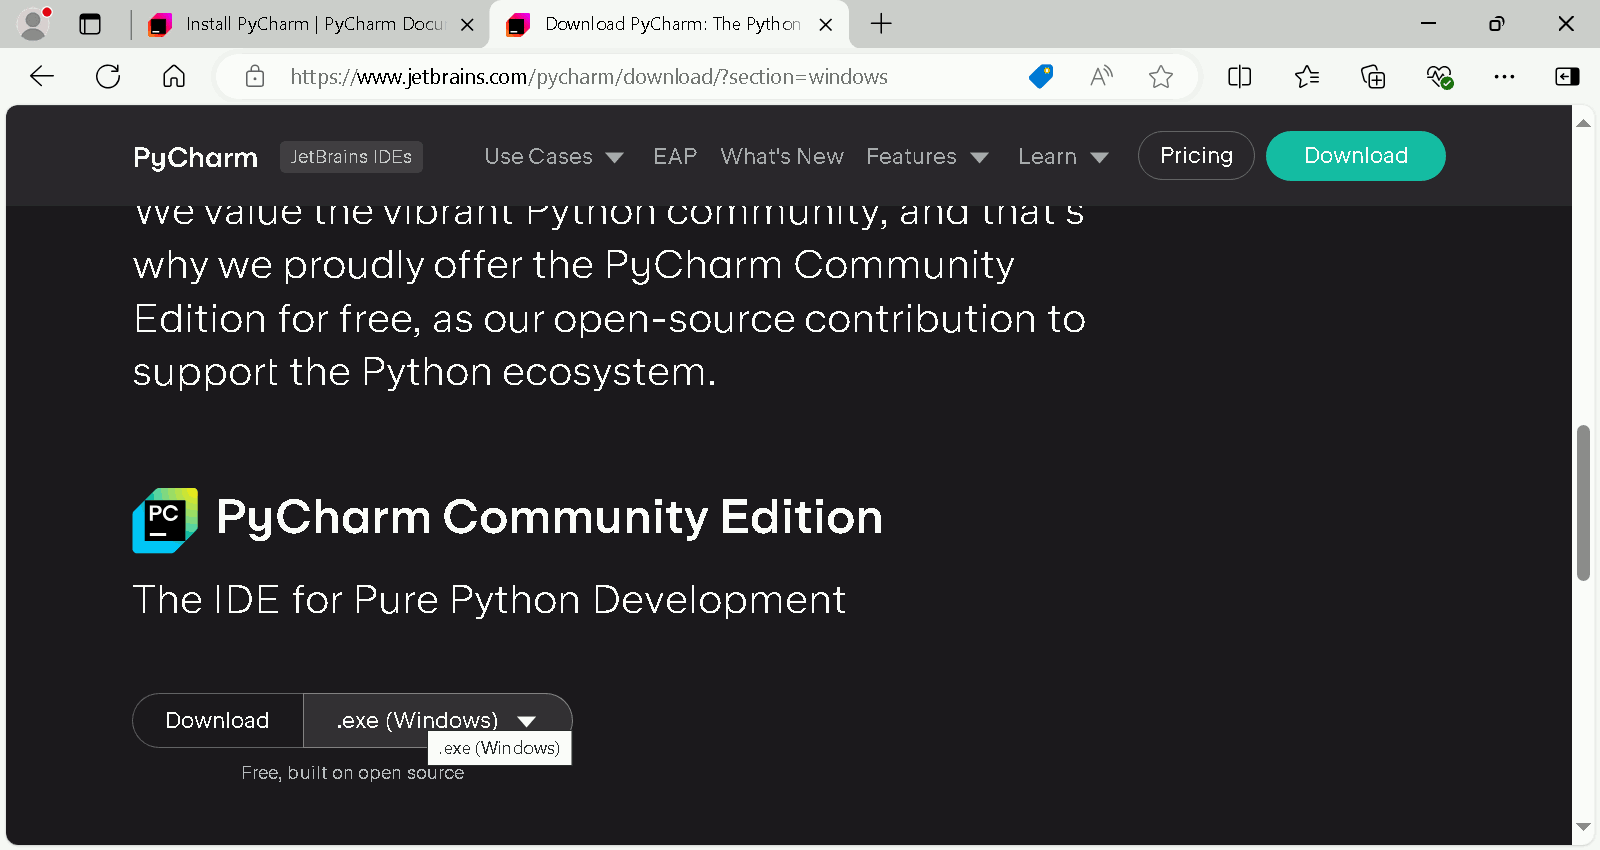
\includegraphics[width=0.47\linewidth]{\currentDir/installingPyCharmWindows02download}}}%
%
\\[10pt]%
%
\subfloat[][%
Selecting the normal \windows\ installer for the \pycharm\ Community Edition.%
\label{fig:installingPyCharmWindows03download}%
]{\tightbox{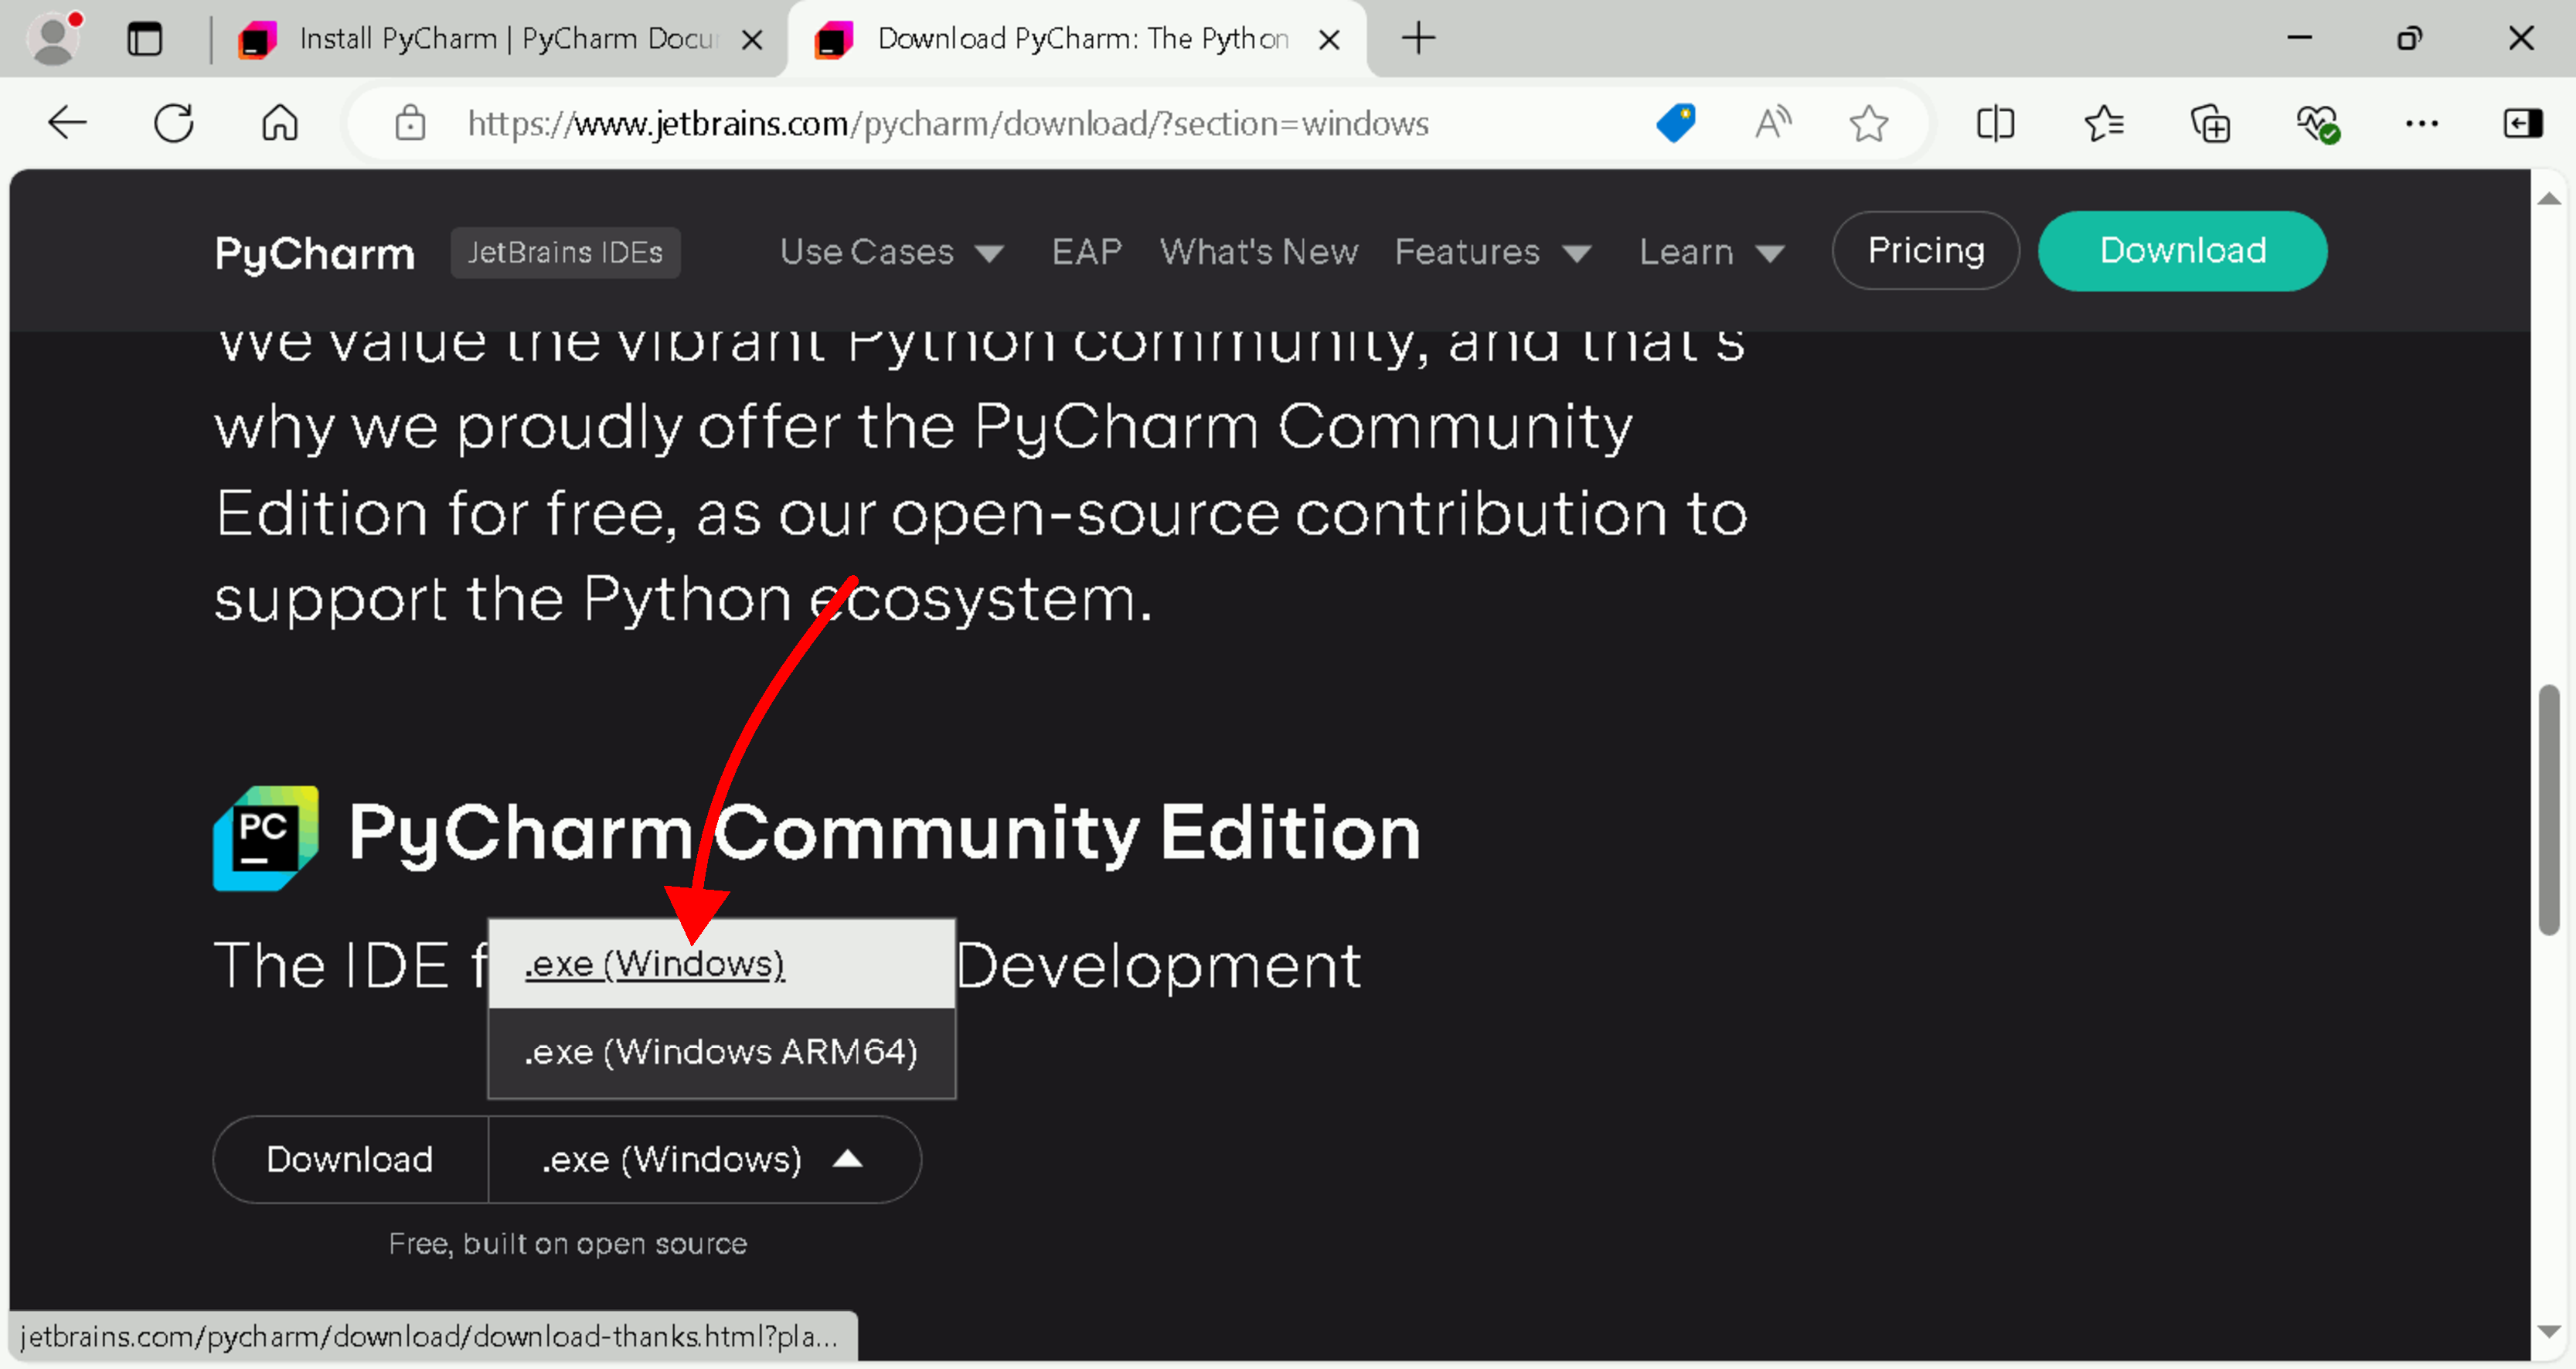
\includegraphics[width=0.47\linewidth]{\currentDir/installingPyCharmWindows03download}}}%
%
\hfill%
%
\subfloat[][%
The download is starting.%
\label{fig:installingPyCharmWindows04download}%
]{\tightbox{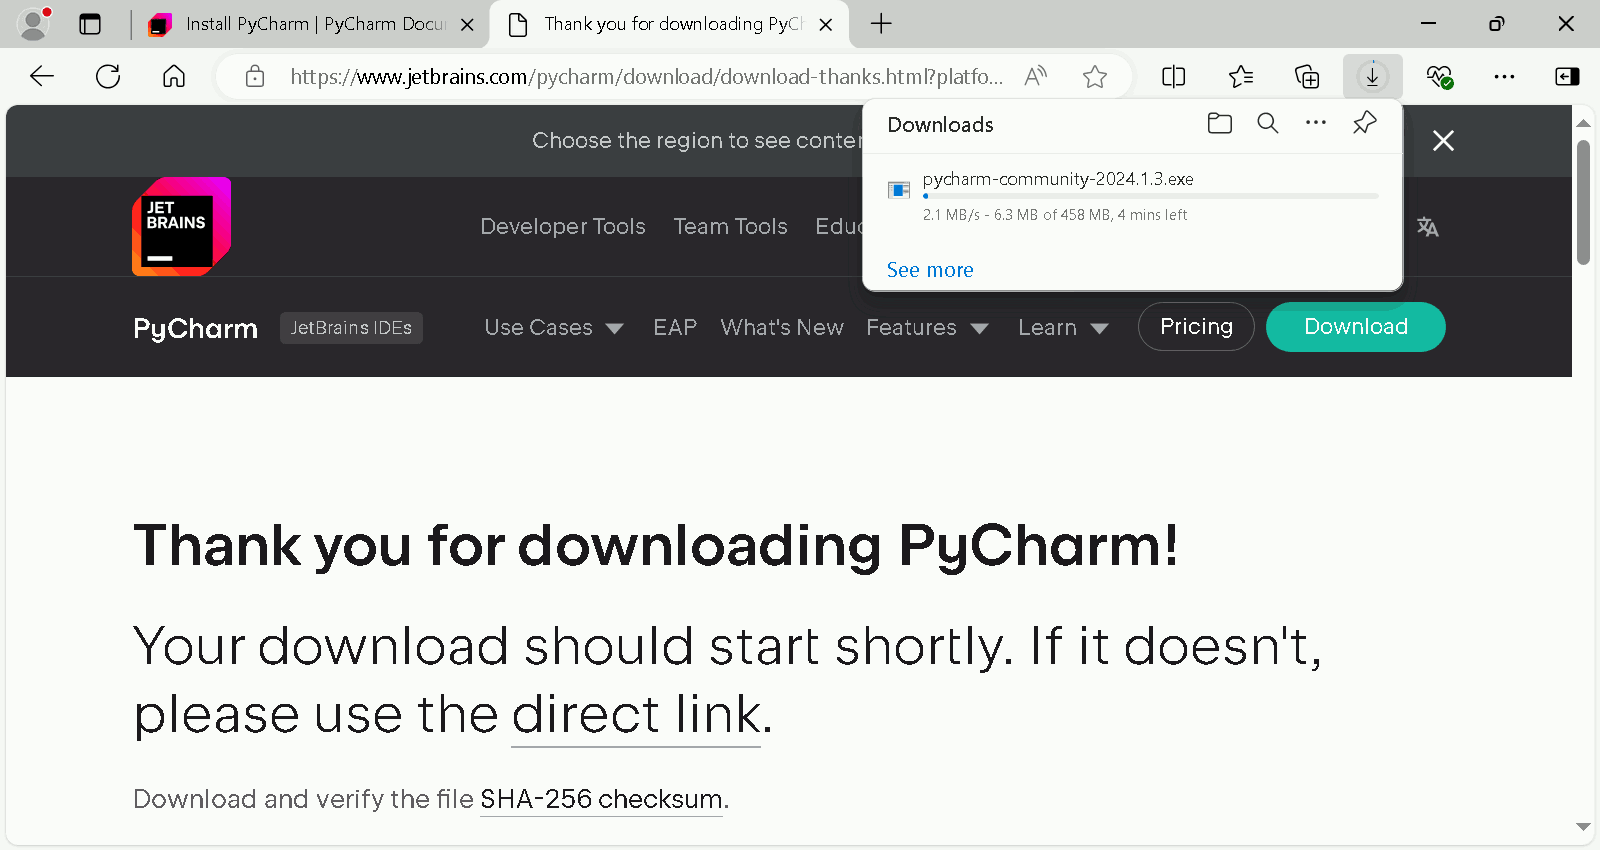
\includegraphics[width=0.47\linewidth]{\currentDir/installingPyCharmWindows04download}}}%
%
\caption{The installation steps of \pycharm\ under \windows.}%
\label{fig:installingPyCharmWindowsA}%
%
\end{figure}%
\begin{figure}%
\ContinuedFloat%
%
\subfloat[][%
The download is completed. We click \keys{Open file}.%
\label{fig:installingPyCharmWindows05runInstaller}%
]{\tightbox{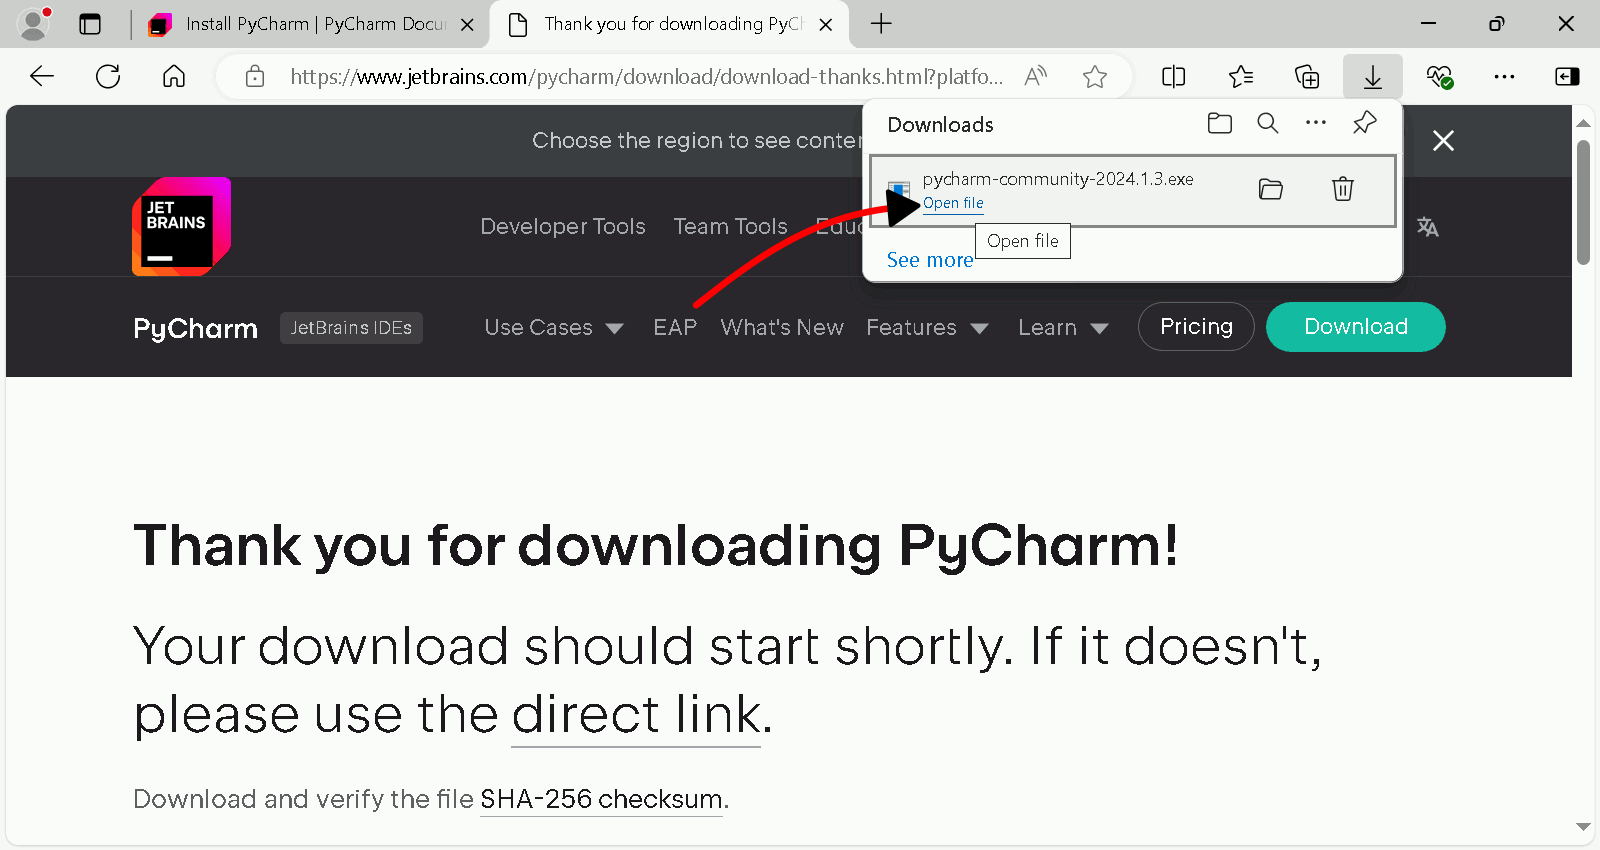
\includegraphics[width=0.47\linewidth]{\currentDir/installingPyCharmWindows05runInstaller}}}%
%
\hfill%
%
\subfloat[][%
The installer is starting.%
\label{fig:installingPyCharmWindows06runInstaller}%
]{\tightbox{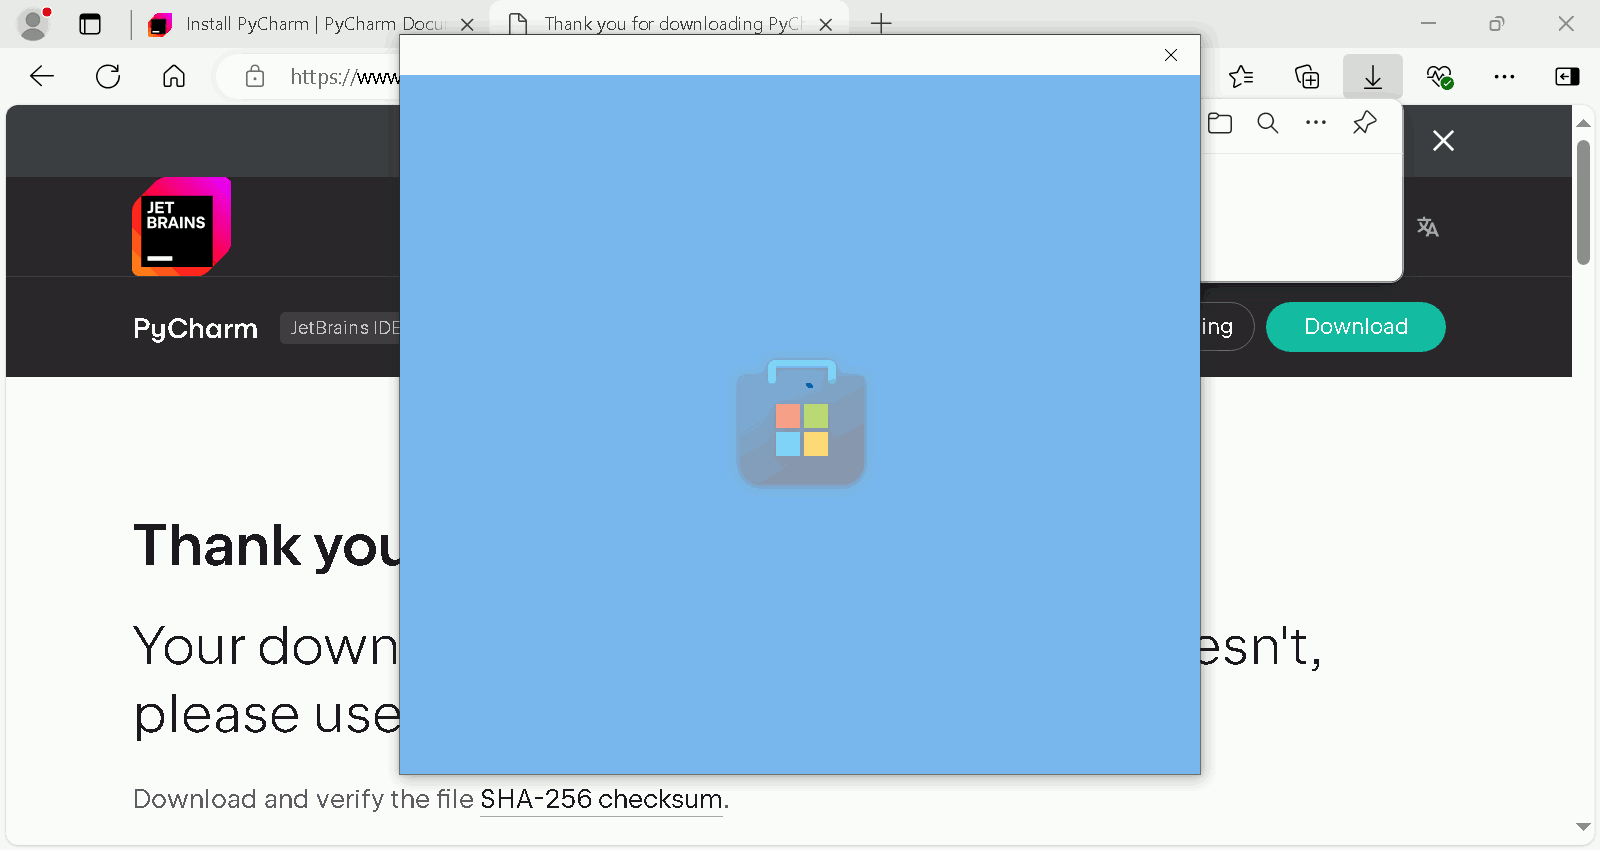
\includegraphics[width=0.47\linewidth]{\currentDir/installingPyCharmWindows06runInstaller}}}%
%
\\[10pt]%
%
\subfloat[][%
The installer is starting.%
\label{fig:installingPyCharmWindows07runInstaller}%
]{\tightbox{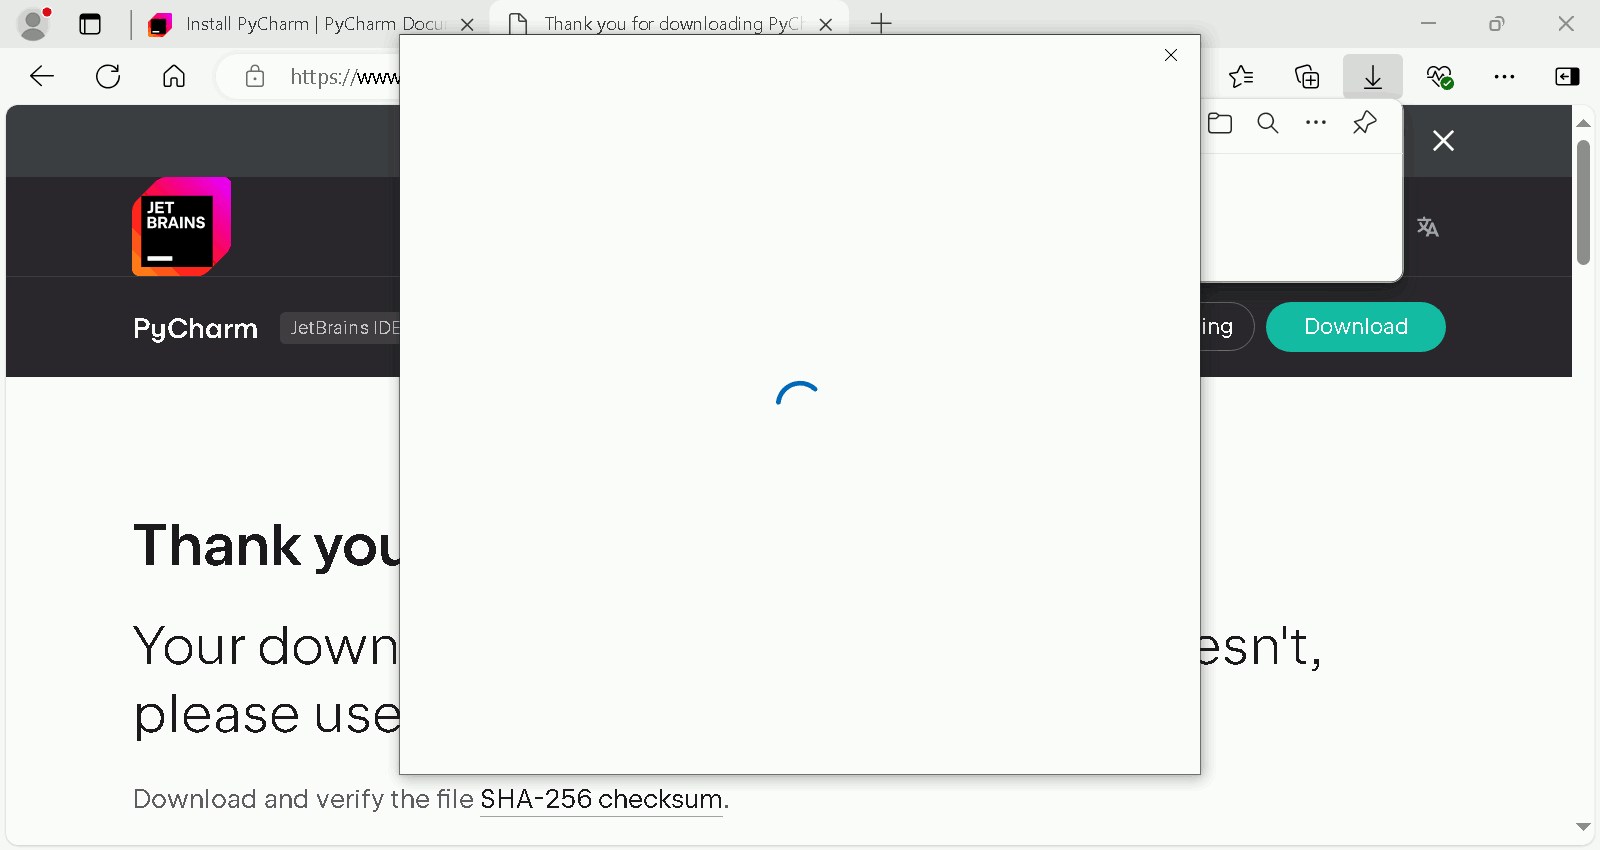
\includegraphics[height=3.75cm]{\currentDir/installingPyCharmWindows07runInstaller}}}%
%
\hfill\hfill%%
%
\subfloat[][%
We do want to install, so click \keys{Yes}.%
\label{fig:installingPyCharmWindows08runInstaller}%
]{\tightbox{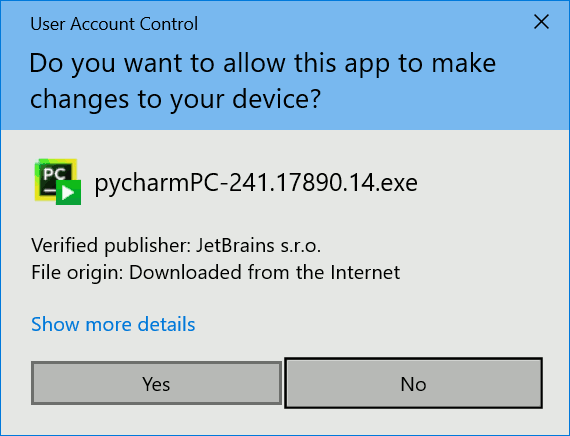
\includegraphics[height=3.75cm]{\currentDir/installingPyCharmWindows08runInstaller}}}%
\hfill\strut%
%
\\[10pt]%
%
\subfloat[][%
The welcome screen of the installer. We click \keys{Next}.%
\label{fig:installingPyCharmWindows09installation}%
]{\tightbox{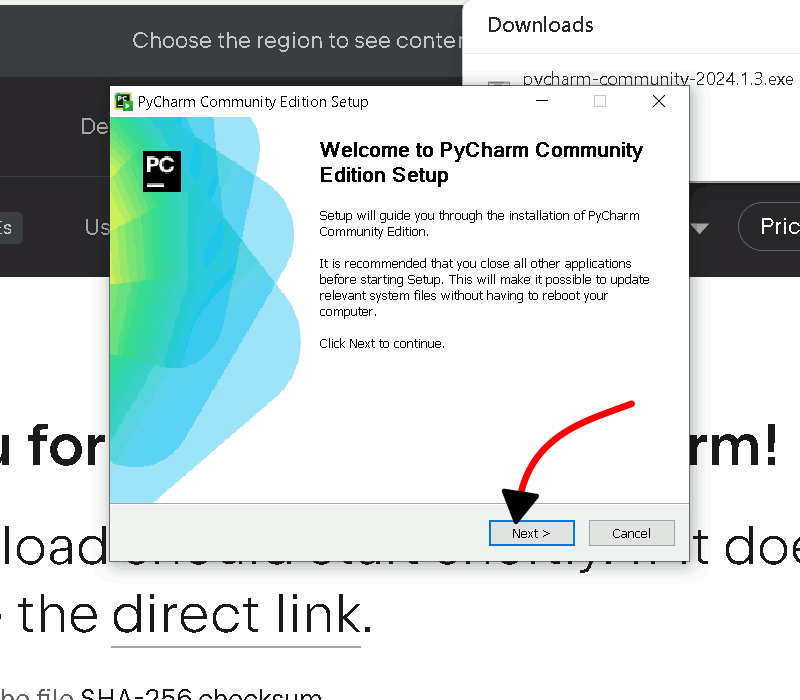
\includegraphics[height=4cm]{\currentDir/installingPyCharmWindows09installation}}}%
%
\hfill%
%
\subfloat[][%
The installation folder selection. We click \keys{Next}.%
\label{fig:installingPyCharmWindows10installation}%
]{\tightbox{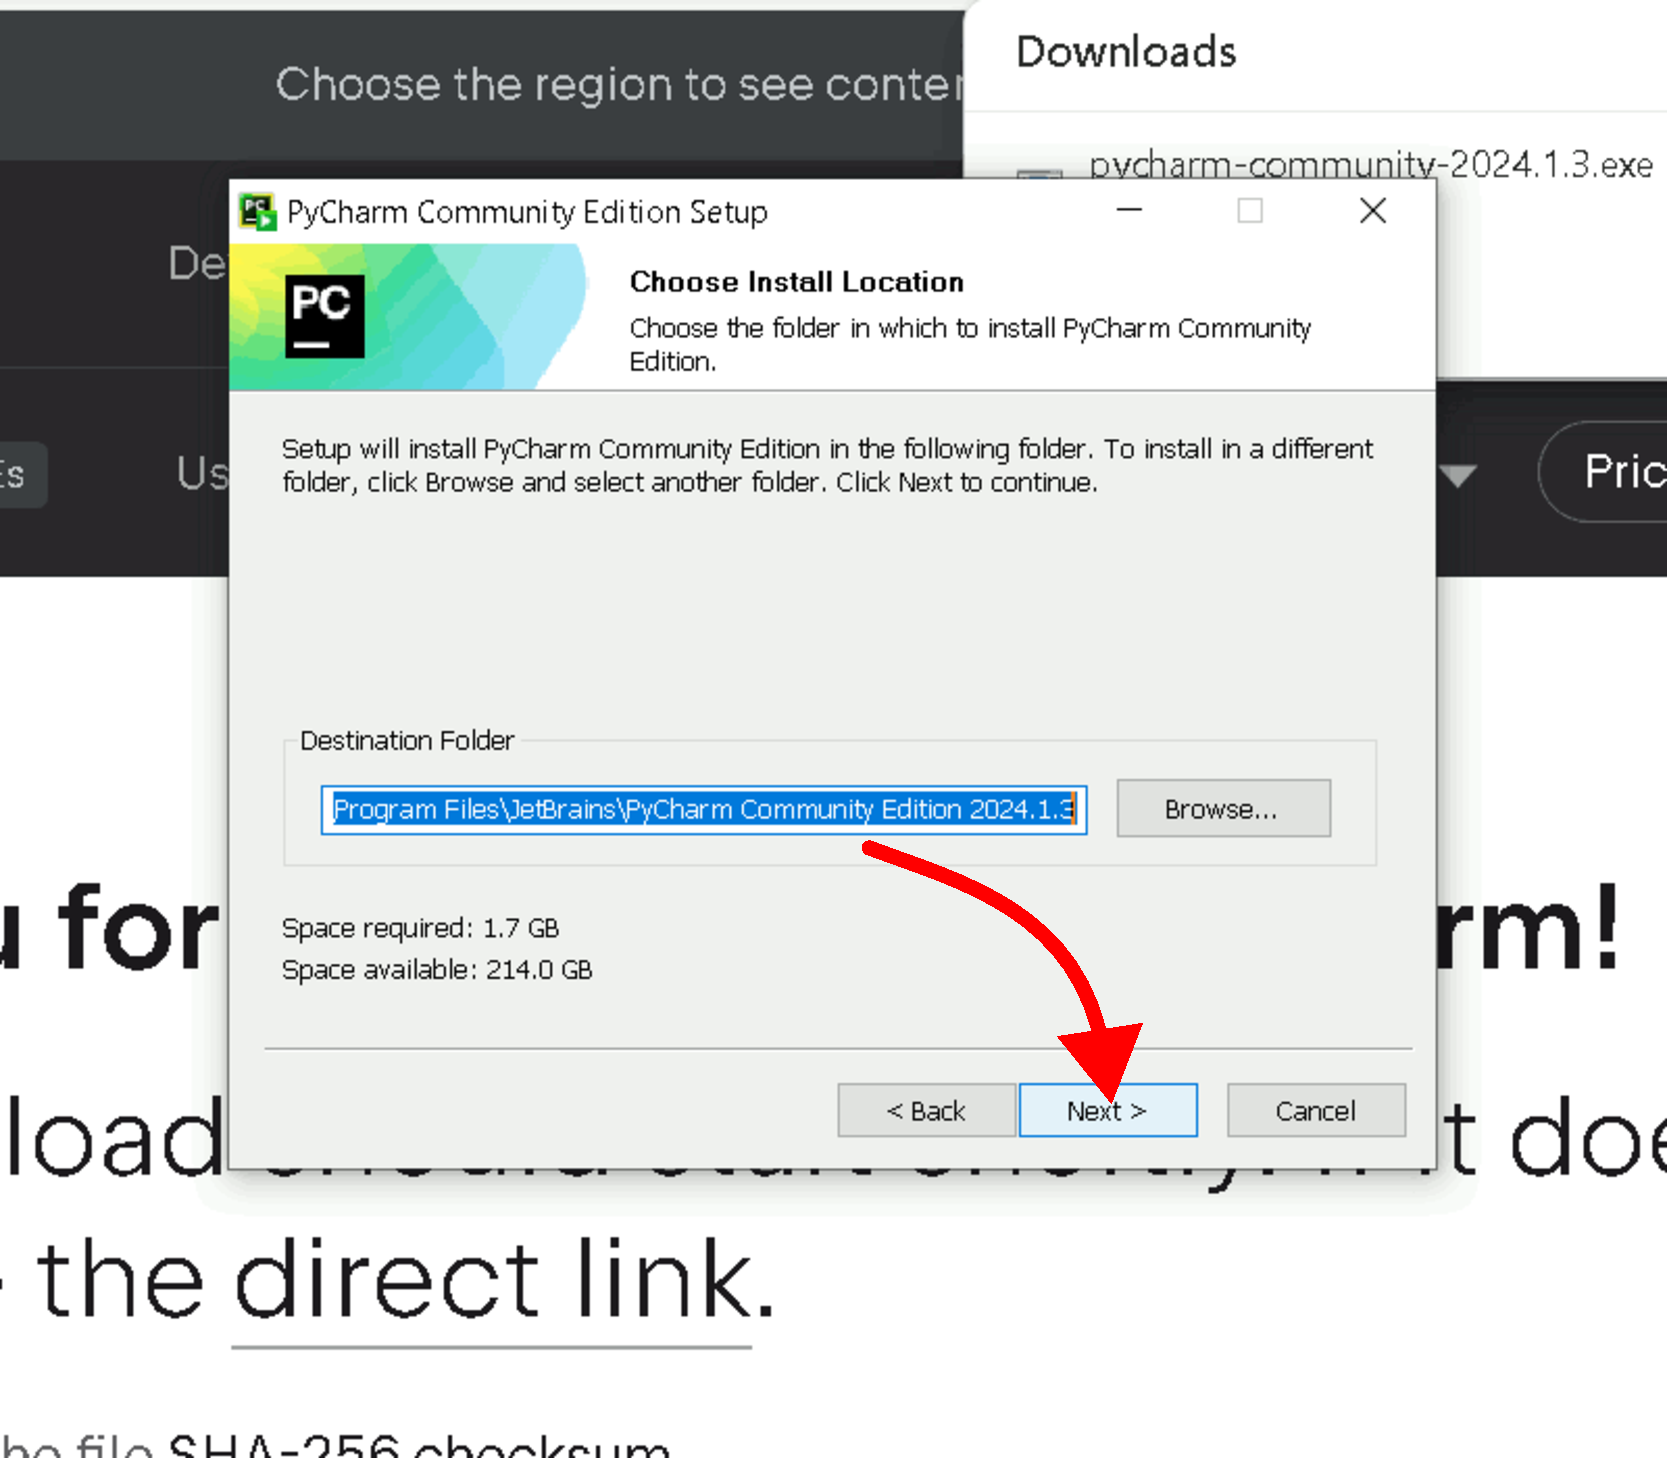
\includegraphics[height=4cm]{\currentDir/installingPyCharmWindows10installation}}}%
%
\hfill%
%
\subfloat[][%
The installation options. We can click \keys{Next}.%
\label{fig:installingPyCharmWindows11installation}%
]{\tightbox{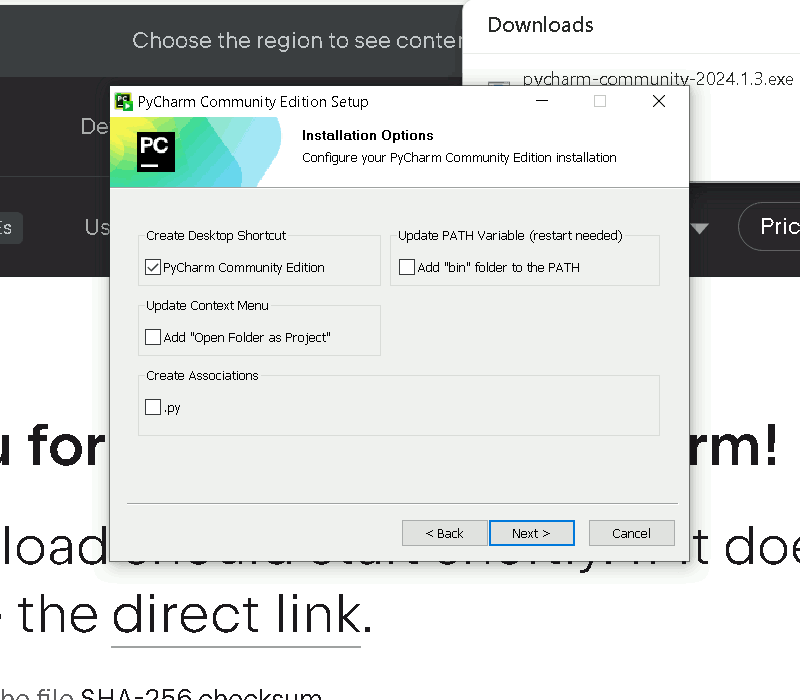
\includegraphics[height=4cm]{\currentDir/installingPyCharmWindows11installation}}}%
%
\\[10pt]%
%
\subfloat[][%
The start menu folder choose dialog. We click \keys{Install}.%
\label{fig:installingPyCharmWindows12installation}%
]{\tightbox{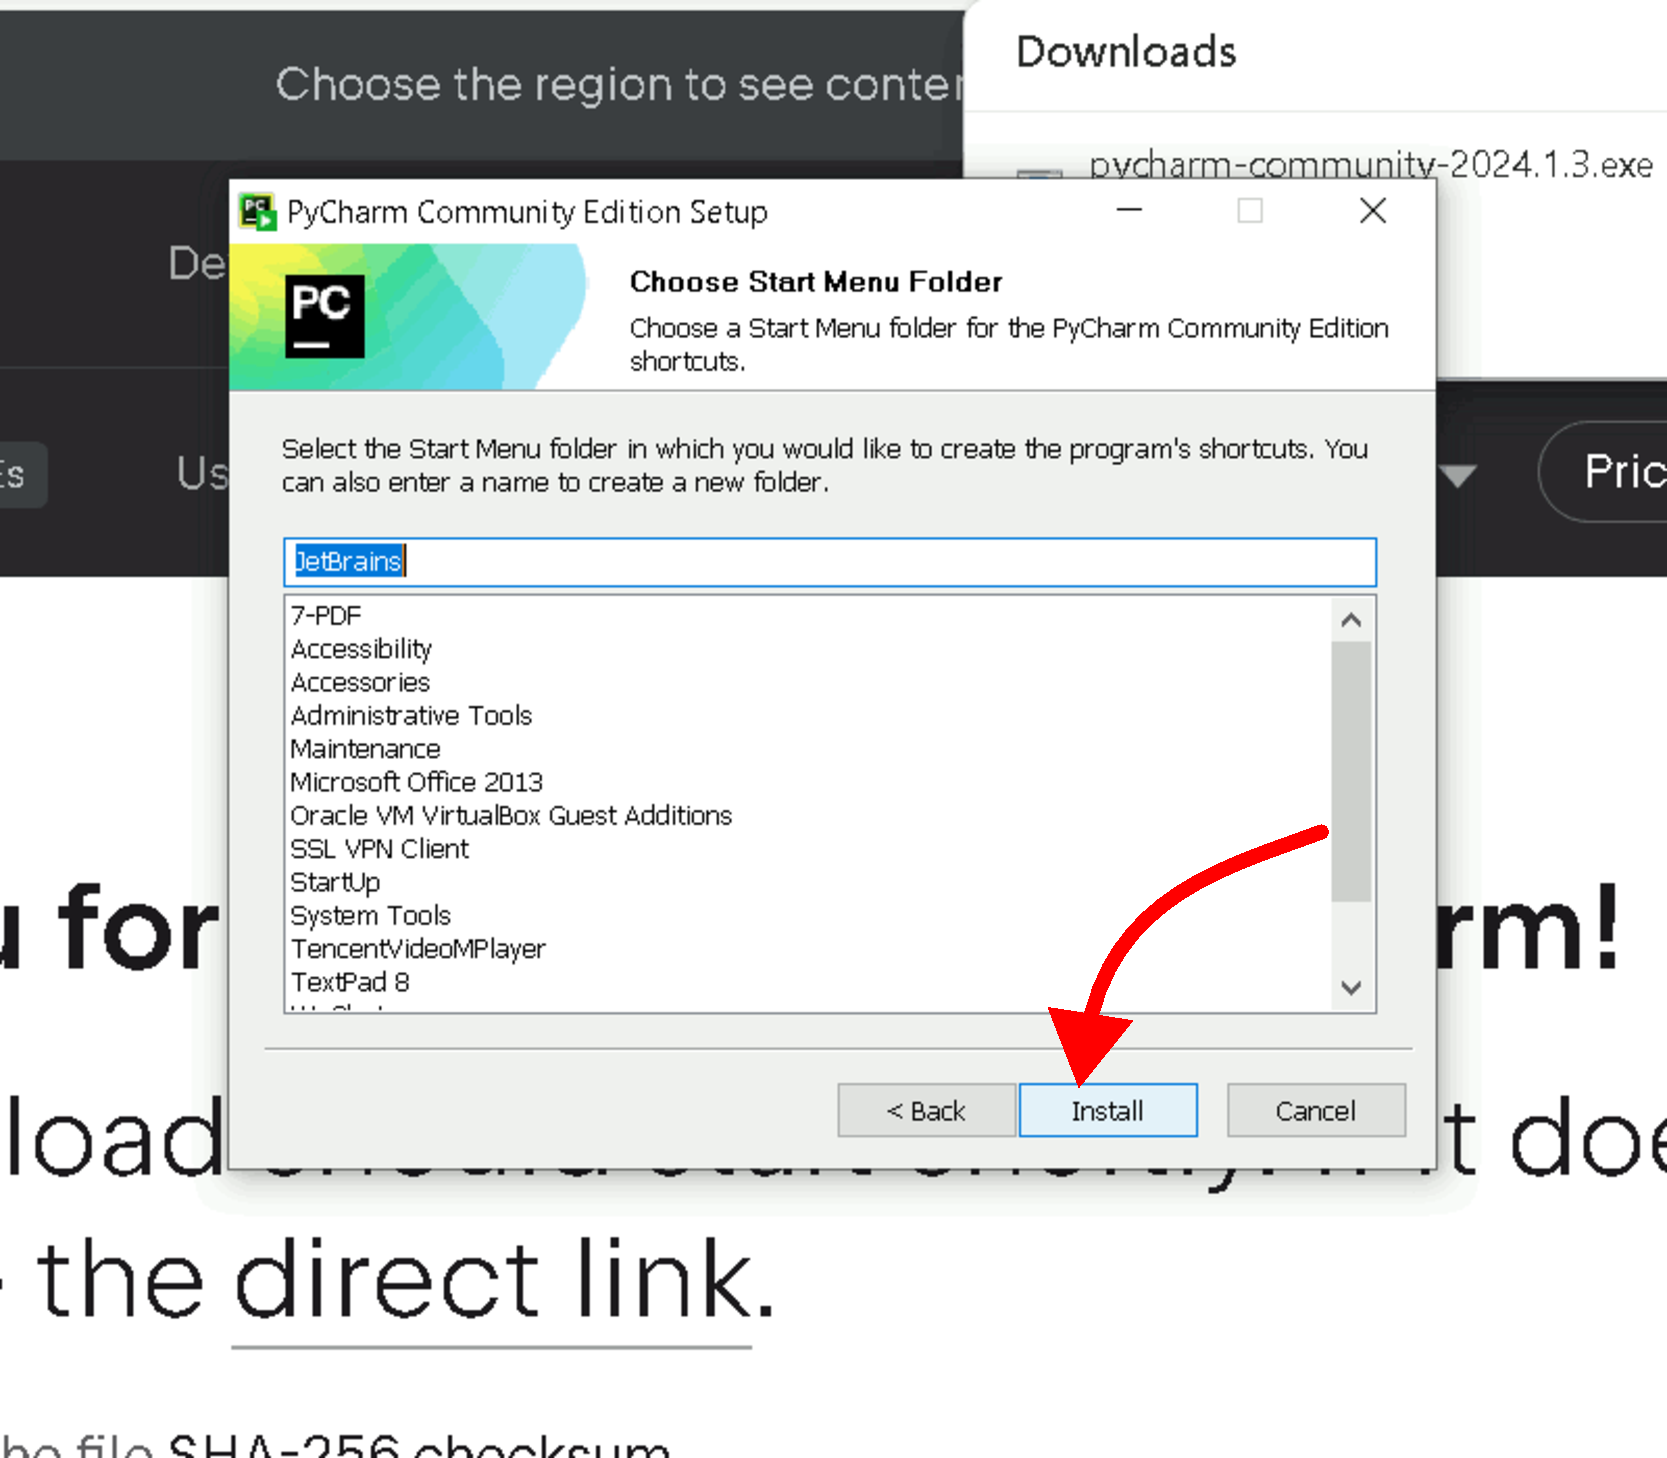
\includegraphics[height=4cm]{\currentDir/installingPyCharmWindows12installation}}}%
%
\hfill%
%
\subfloat[][%
The install process starts.%
\label{fig:installingPyCharmWindows13installation}%
]{\tightbox{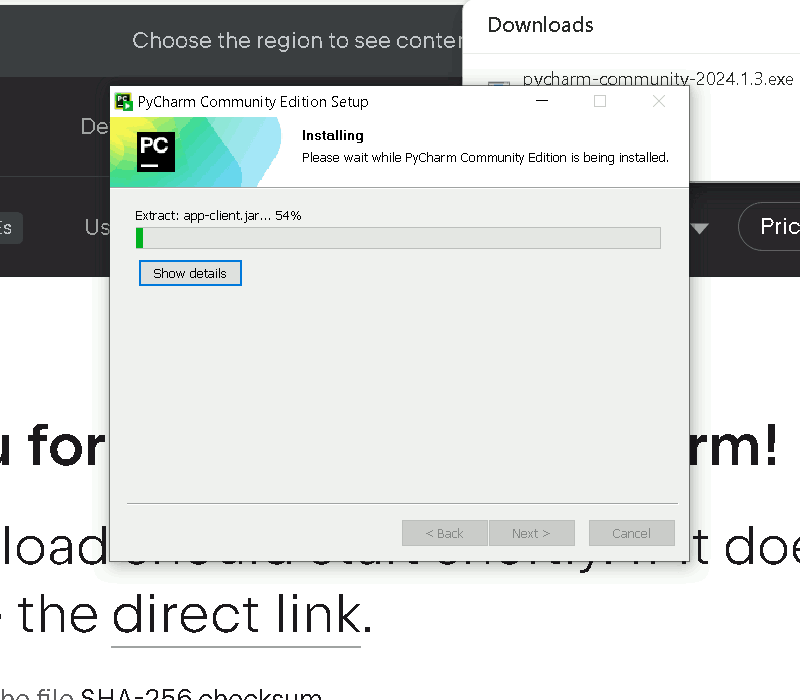
\includegraphics[height=4cm]{\currentDir/installingPyCharmWindows13installation}}}%
%
\hfill%
%
\subfloat[][%
The installation is finished. Select ``Run PyCharm Community Edition'' and click \keys{Finish}.%
\label{fig:installingPyCharmWindows14installation}%
]{\tightbox{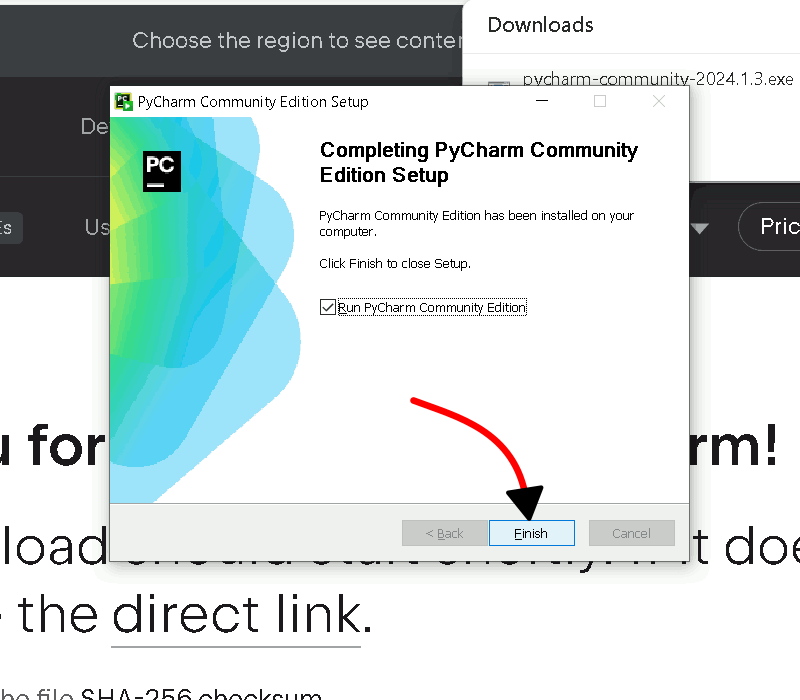
\includegraphics[height=4cm]{\currentDir/installingPyCharmWindows14installation}}}%
%
\caption{The installation steps of \pycharm\ under \windows~(continued).}%
\label{fig:installingPyCharmWindowsB}%
%
\end{figure}%
%
\begin{figure}%
\ContinuedFloat%
\centering%
%
\strut\hfill\strut%
\subfloat[][%
The welcome screen of \pycharm.%
\label{fig:installingPyCharmWindows15running}%
]{\tightbox{
\includegraphics[width=0.4\linewidth]{\currentDir/installingPyCharmWindows15running}}}%
%
\strut\hfill\strut\strut\hfill\strut%%
%
\subfloat[][%
We read the user agreement, confirm that we read it, and click \keys{Continue}.%
\label{fig:installingPyCharmWindows16running}%
]{\tightbox{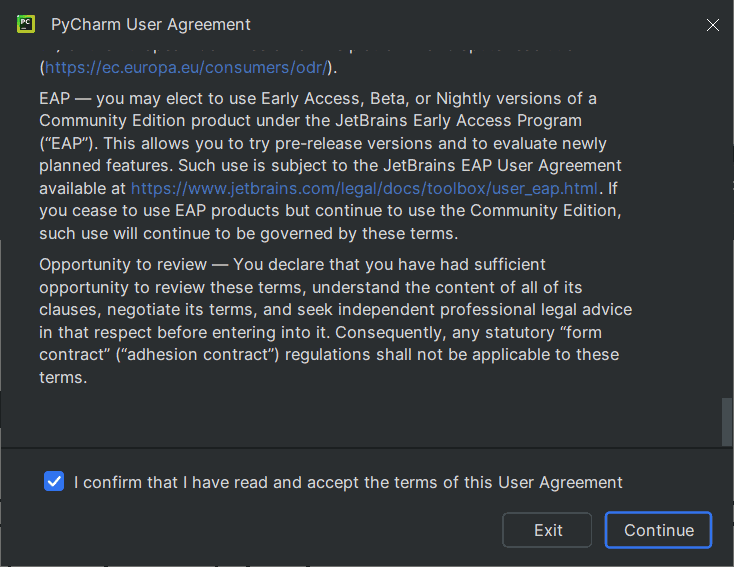
\includegraphics[width=0.4\linewidth]{\currentDir/installingPyCharmWindows16running}}}%
\strut\hfill\strut%
%
\\[10pt]%
%
\strut\hfill\strut%
\subfloat[][%
We do not want to send any data and click \keys{Don't Send}.%
\label{fig:installingPyCharmWindows17running}%
]{\tightbox{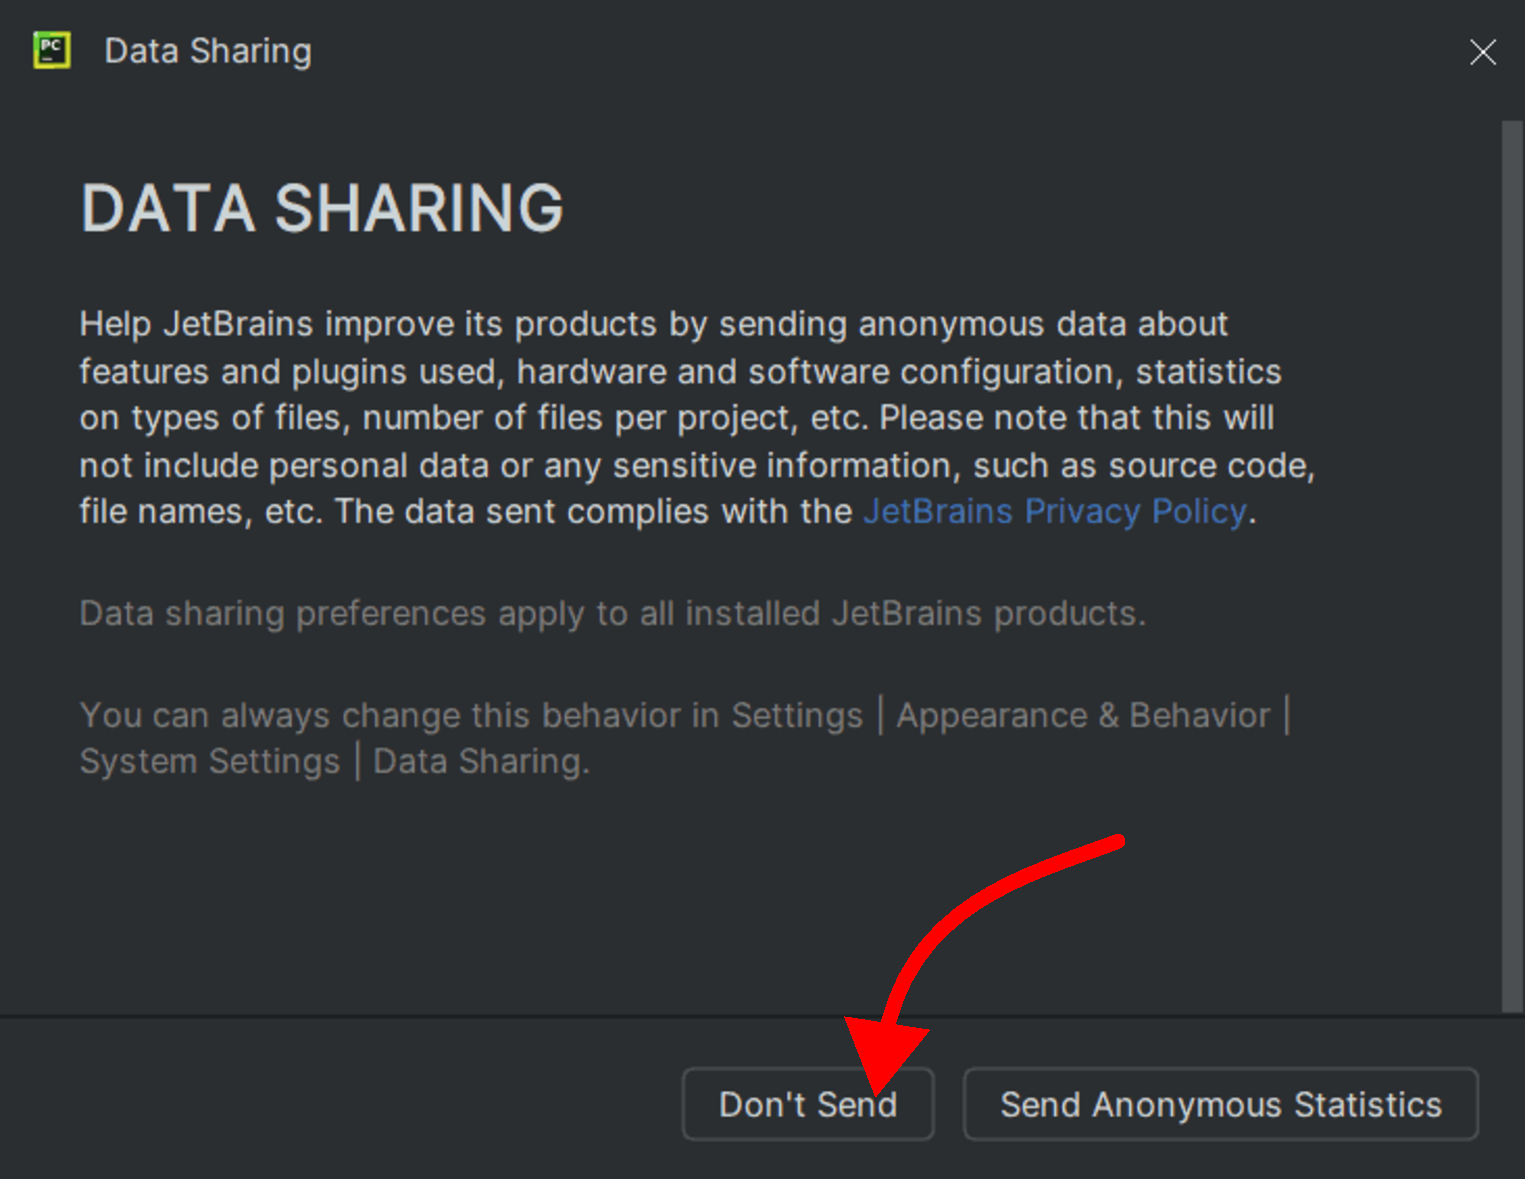
\includegraphics[width=0.4\linewidth]{\currentDir/installingPyCharmWindows17running}}}%
%
\strut\hfill\strut\strut\hfill\strut%%
%
\subfloat[][%
Finally, \pycharm\ is ready to use.%
\label{fig:installingPyCharmWindows18running}%
]{\tightbox{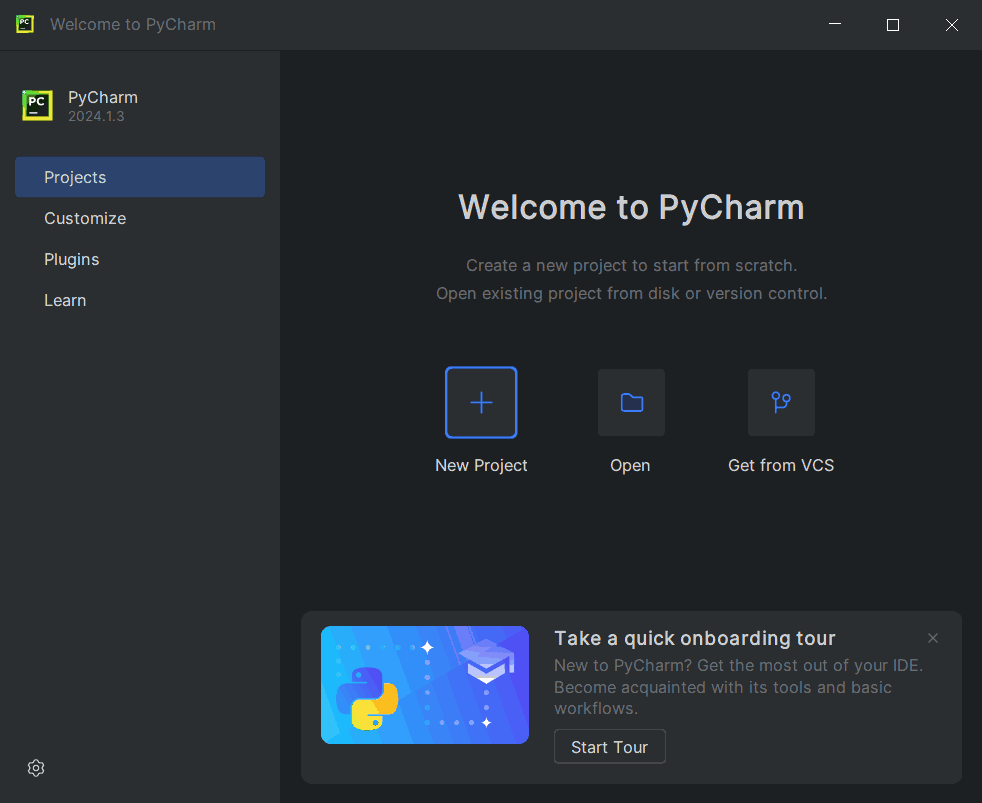
\includegraphics[width=0.4\linewidth]{\currentDir/installingPyCharmWindows18running}}}%
\strut\hfill\strut%
%
\caption[]{The installation steps of \pycharm\ under \windows~(continued).}%
\label{fig:installingPyCharmWindowsC}%
\end{figure}%
%
The process of installing \pycharm\ under \windows\ is illustrated in \cref{fig:installingPyCharmWindowsA}.
You first need to download the \pycharm\ Community Edition installation executable from \url{https://www.jetbrains.com/pycharm/download}.
Make sure to download the Community Edition and nothing else, as shown in \cref{fig:installingPyCharmWindows01download,fig:installingPyCharmWindows02download,fig:installingPyCharmWindows03download}.
Once the installer is downloaded, you start it and confirm that you wish to install \pycharm, as illustrated in \cref{fig:installingPyCharmWindows05runInstaller,fig:installingPyCharmWindows06runInstaller,fig:installingPyCharmWindows07runInstaller,fig:installingPyCharmWindows08runInstaller}.
As \cref{fig:installingPyCharmWindows09installation,fig:installingPyCharmWindows10installation,fig:installingPyCharmWindows11installation} show, the installation setup process is more or less automated, we just need to click \keys{Next} here and there and finally click \keys{Install}~(\cref{fig:installingPyCharmWindows12installation}).
After the installation completes, we run \pycharm\ for the first time.
Now we need to agree to the user agreement~(\cref{fig:installingPyCharmWindows16running}) and should probably choose that we do not with to send any information about our \pycharm\ usage out~(\cref{fig:installingPyCharmWindows17running}).
Finally, as sketched in \cref{fig:installingPyCharmWindows18running}, we have a running and ready \pycharm\ \pgls{IDE}.%
%
\endhsection%
%
